\section{Results}

All experiments can be reproduced using the \texttt{GAIL\_testing.ipynb} notebook in \href{https://github.com/nicholasRenninger/GAIL-Formal_Methods}{my github repo}. To run it, you will need to install docker, then build my docker image using the Makefile / Dockerfile I wrote, and then run it using the provided bash scripts. This will open a jupyter notebook and tensorboard in the container and handle the networking between the host and the container. It has been tested to work on both macOS and linux, on machines both with and without GPUs.

To see gifs of both the expert and GAIL policy in the gridworld, you can visit the main page of the github repo.

The results of the learning process are presented here. Shown in Figs. \ref{fig: expert_rew} and \ref{fig: expert_loss} are the episodic reward and learning curve for the PPO2 RL expert training process. As is quite evident, the PPO2 agent trained well and quickly, needing only 200k environmental interations total to learn a nearly perfect policy. The expert policy had an approximate mean reward of 0.97 $\pm$ 0.01 -- a nearly perfect result -- when simulated after learning. Looking at the videos of the agent's interaction, the PPO2 expert was never observed to do anything besides quickly and efficiently reach the goal safely.

\begin{figure}[htbp]
\centerline{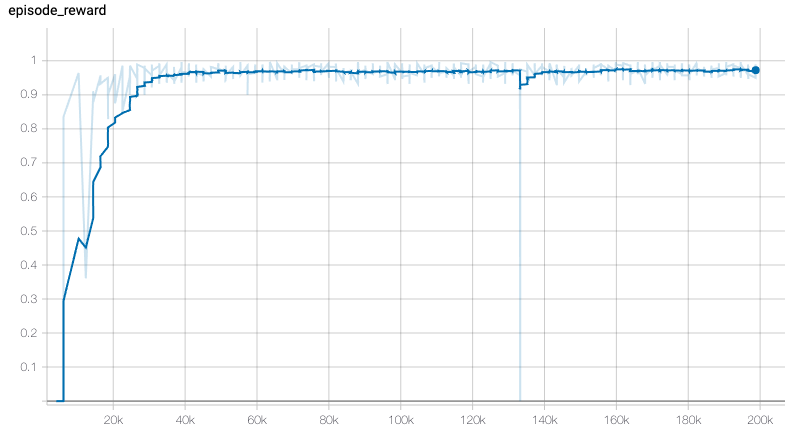
\includegraphics[width=\linewidth]{Figures/expert_reward.png}}
\caption{The final PPO2 training episodic, non-discounted reward as a function of training step.}
\label{fig: expert_rew}
\end{figure}

\begin{figure}[htbp]
\centerline{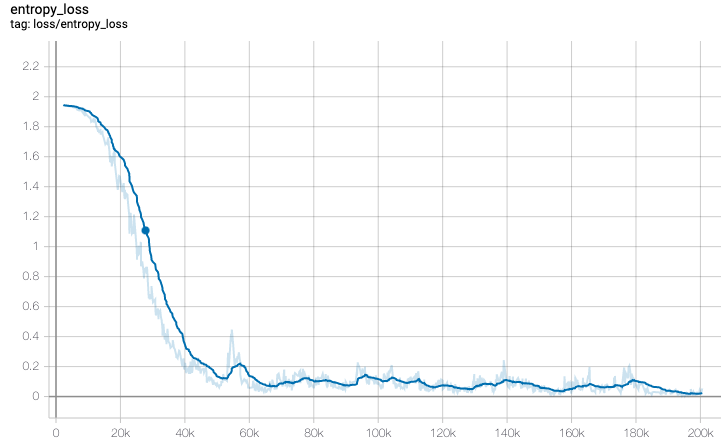
\includegraphics[width=\linewidth]{Figures/expert_loss.png}}
\caption{The final PPO2 entropy loss as a function of training step.}
\label{fig: expert_loss}
\end{figure}

The GAIL training results were, on the other hand, extremely frustrating. Despite weeks of debugging and working with the package maintainers, it was discovered that the GAIL learner has some pernicious bugs with the handling of the MPI based training environment parallelization that have not been squashed. Thus, as can be seen in Figs. \ref{fig: gail_rew} - \ref{fig: gail_policy_rew}, GAIL never ended up learning the proper thing. As can be seen specifically in Figs \ref{fig: gail_discrim_loss} and \ref{fig: gail_policy_rew}, the GAIL training was obviously having problems even with the "best" hyperparameters chosen. The dicriminator loss never reached 0, even after 1M iterations, and the policy gradient reward signal stagnated over time instead of improving, despite the fact the TRPO RL engine in GAIL should guarantee monotonic improvements in the solution quality. GAIL never received more than 0 reward.

\begin{figure}[htbp]
\centerline{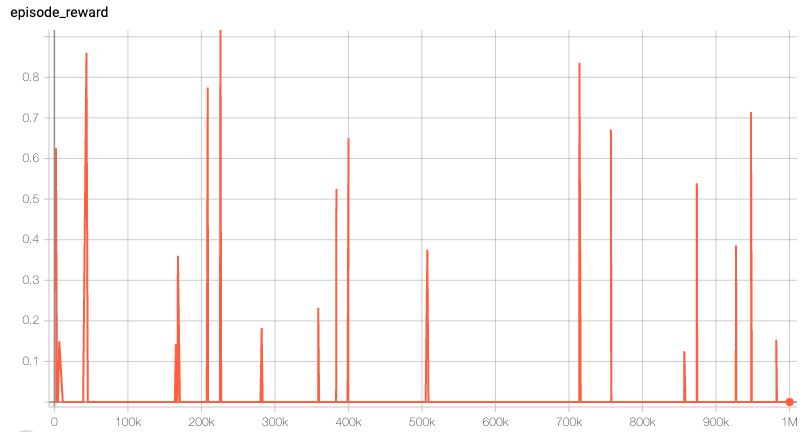
\includegraphics[width=\linewidth]{Figures/gail_episode_reward.png}}
\caption{The final GAIL episodic, non-discounted reward as a function of training step.}
\label{fig: gail_rew}
\end{figure}

\begin{figure}[htbp]
\centerline{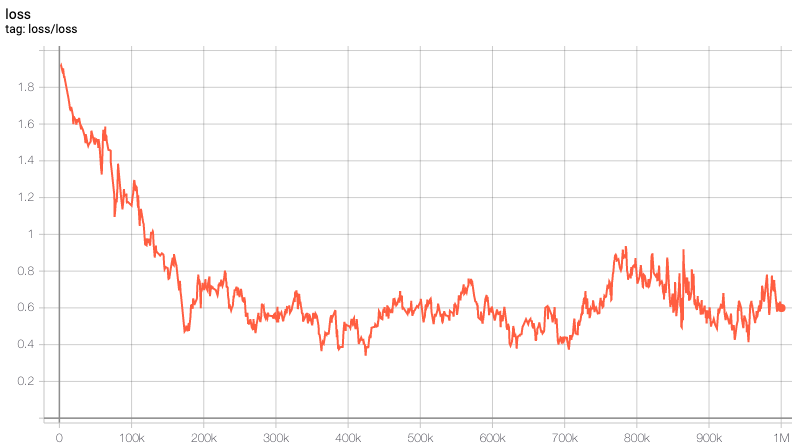
\includegraphics[width=\linewidth]{Figures/gail_discriminator_loss.png}}
\caption{The final GAIL discriminator classification loss as a function of training step.}
\label{fig: gail_discrim_loss}
\end{figure}

\begin{figure}[htbp]
\centerline{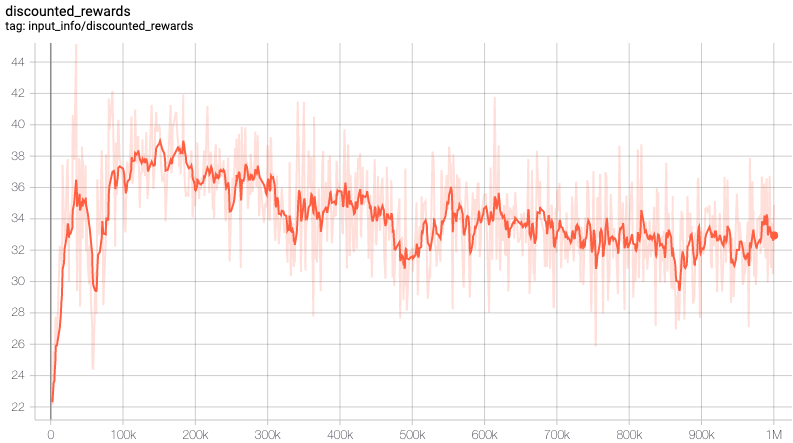
\includegraphics[width=\linewidth]{Figures/gail_policy_net_reward_signal.png}}
\caption{The final GAIL policy network discounted "reward" signal from the descriminator as a function of training step.}
\label{fig: gail_policy_rew}
\end{figure}

When the expert was moved to a new domain, shown in Fig. \ref{fig: ppo2_generlaization}, its policy was brittle and it did not generalize at all.

\begin{figure}[htbp]
\centerline{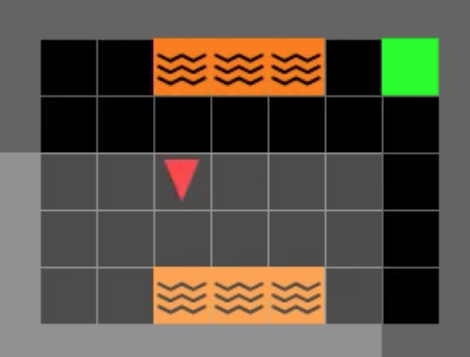
\includegraphics[width=\linewidth]{Figures/new_env.png}}
\caption{The final PPO2 policy network trying (and failing) to adapt to a slightly different environment.}
\label{fig: ppo2_generlaization}
\end{figure}